%
%
\comment{
\begin{itemize}
	\item we need to do both width adaptation and clock-domain crossing
	\item draw out the schematic of FabricPort input/output
	\item how to determine VC? each message class has only one VC to choose from
	\item only one physical port can be connected to each FabricPort unless we can tolerate throughput degradation
	\item multiple VCs can still share the output mux ports to the fabric interconnect
\end{itemize}
}
%
%

%---------------------------------------------------------------------------------------------------------
\subsection{Packet Format}
%---------------------------------------------------------------------------------------------------------


%
\figvs{1}{packet_format}{}{NoC packets consist of a head flit and zero-or-more body flits. The figure shows flits for a 16-node 150-bit-width NoC with 2 VCs. Each flit has control data to indicate whether this flit is valid, and if it is the head or tail flit (or both for a 1-flit packet). Additionally each flit must have the VC number to which it is assigned and a head flit must contain the destination address.}
%


Fig.~\ref{packet_format} shows the format of flits on the NoC; each flit is 150~bits making flit width and NoC link width equivalent (as most on-chip networks do)~\cite{dally_book}.
One flit is the smallest unit that can be sent over the NoC, indicating that the NoC will be used for coarse-grained wide datapath transfers.
This packet format puts no restriction on the number of flits that form a packet; each flit has two bits for ``head" and ``tail" to indicate the flit at the start of a packet, and the flit at the end of a packet.
The VC identifier is required for proper virtual-channel flow control, and finally, the head flit must also contain the destination address so that the NoC knows where to send the packet.
The remaining bits are data, making the control overhead quite small in comparison; for a 4-flit packet, control bits make up 3\% of transported data.


%
%---------------------------------------------------------------------------------------------------------
\subsection{FabricPort Functionality}
%---------------------------------------------------------------------------------------------------------
%

Each NoC port can sustain a maximum input bandwidth of 22.5~GB/s; however, this is done at the high frequency of 1.2~GHz for our NoC.
The main purpose of the FabricPort is therefore to give the FPGA fabric access to that communication bandwidth, at the range of frequencies at which FPGAs normally operate.
How does one connect a module configured from the FPGA fabric to the embedded NoC running at a different width and frequency?

%
\figvs{1}{fp_logical}{}{Data on the FPGA with any protocol can be translated into NoC flits using application-dependent soft logic (translator). A FabricPort then adapts width (1-4 flit width on fabric side and 1 flit width on NoC) and frequency (any frequency on fabric side and 1.2~GHz on NoC side) to inject flits into the NoC.}
%

Fig.~\ref{fp_logical} illustrates the process of conditioning data from any FPGA module to NoC flits, and vice versa.
A very simple translator takes incoming data and appends to it the necessary flit control information.
For most cases, this translator consists only of wires that pack the data in the correct position and sets the valid/head/tail bits from constants.
Once data is formatted into flits, we can send between 0 and 4 flits in each fabric cycle, this is indicated by the valid bit on each flit.
The FabricPort will then serialize the flits, one after the other, and inject the valid ones into the NoC at the NoC's frequency.
When flits are received at the other end of the NoC, the frequency is again bridged, and the width adapted using a FabricPort; then a translator strips control bits and injects the data into the receiving fabric module.

This FabricPort plays a pivotal role in adapting an embedded NoC to function on an FPGA.
We must bridge the width and frequency while making sure that the FabricPort is never a source of throughput reduction; furthermore, the FabricPort must be able to interface to different VCs on the NoC, send/receive different-length packets and respond to backpressure coming from either the NoC or FPGA fabric.
We enumerate the essential properties that this component must have:

\vspace{-0.1cm}

\begin{enumerate}
\setlength\itemsep{-0.33mm}
\item \textbf{Rate Conversion}: Match the NoC bandwidth to the fabric bandwidth. Because the NoC is embedded, it can run \til4\xx faster than the FPGA fabric~\cite{fpt,trets}. We leverage that speed advantage to build a narrow-link-width NoC that connects to a wider but slower FPGA fabric. 
\item \textbf{Stallability}: Accept/send data on every NoC cycle in the absence of stalls, and stall for the exact number of cycles when the fabric/NoC isn't ready to send/receive data (as Fig.~\ref{stall_protocol} shows). The FabricPort itself should never be the source of throughput reduction.
\item \textbf{Virtual Channels}: Read/write data from/to multiple virtual channels in the NoC such that the FabricPort is never the cause for deadlock.
\item \textbf{Packet Length}: Send/receive packets of different lengths.
\item \textbf{Backpressure Translation}: Convert the NoC's credit-based flow-control system into the more FPGA-familiar ready/valid signals.
\end{enumerate}

\vspace{-0.25cm}

%
\figvs{1}{stall_protocol}{}{Waveform of ready/valid signals between soft module $\rightarrow$ FabricPort input, or FabricPort output $\rightarrow$ soft module. After ``ready" signal becomes low, the receiver must accept one more cycle of valid data (data 2) after which the sender will have processed the ``ready" signal and stopped sending more valid data.}
%

%---------------------------------------------------------------------------------------------------------
\subsection{FabricPort Circuitry}
%---------------------------------------------------------------------------------------------------------


\begin{figure*}[t]
\centering
\subfloat[FabricPort input: from the FPGA fabric to the embedded NoC.]{
   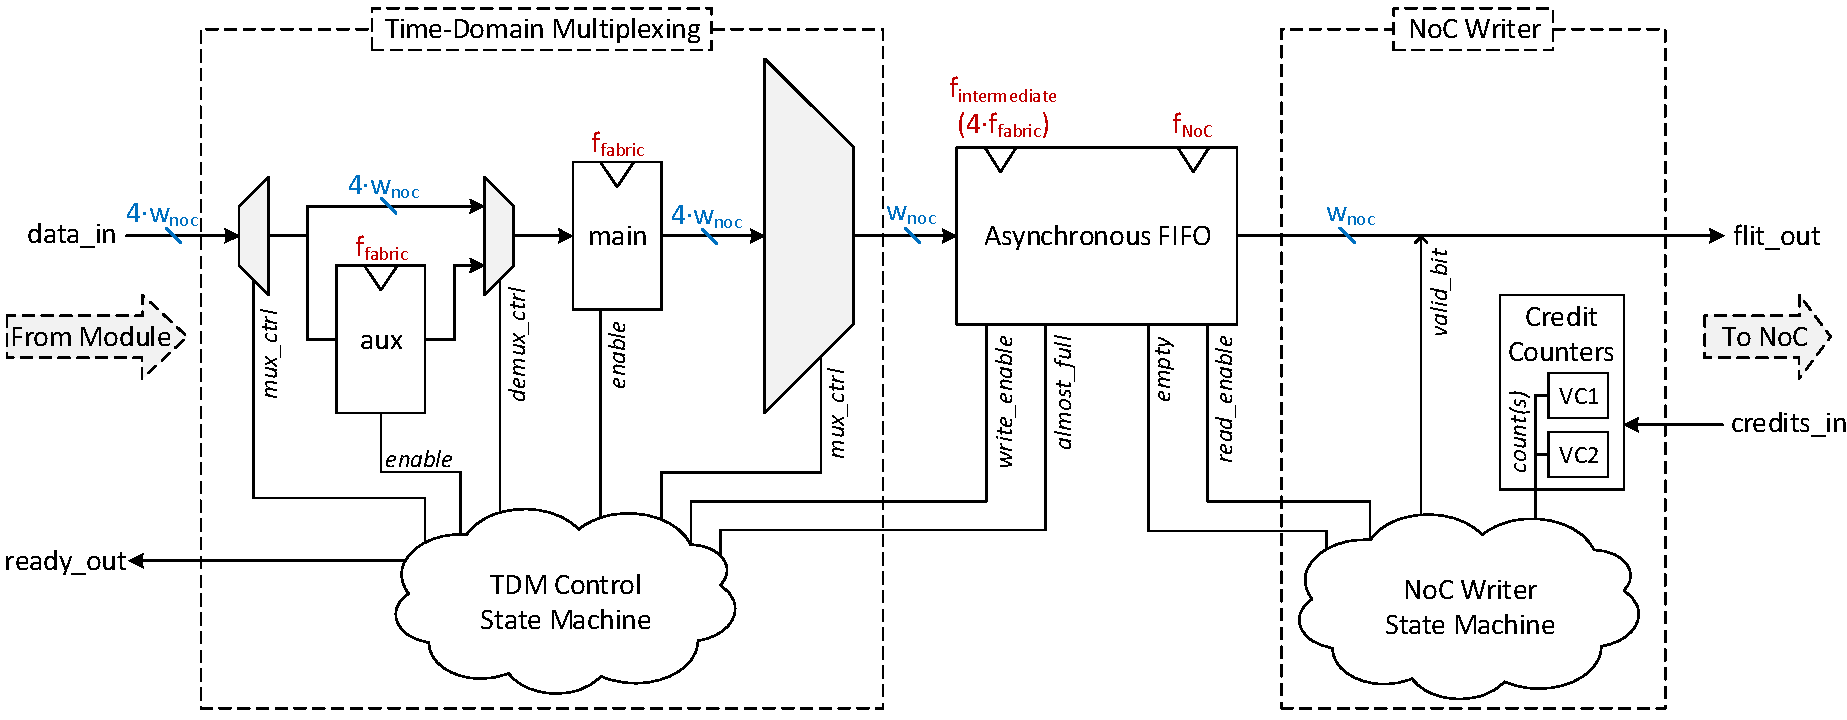
\includegraphics[width=2\columnwidth,keepaspectratio]{images/fpin_detail}
   \label{fpin}
 }
 \\
\subfloat[FabricPort output: from the embedded NoC to the FPGA fabric.]{
   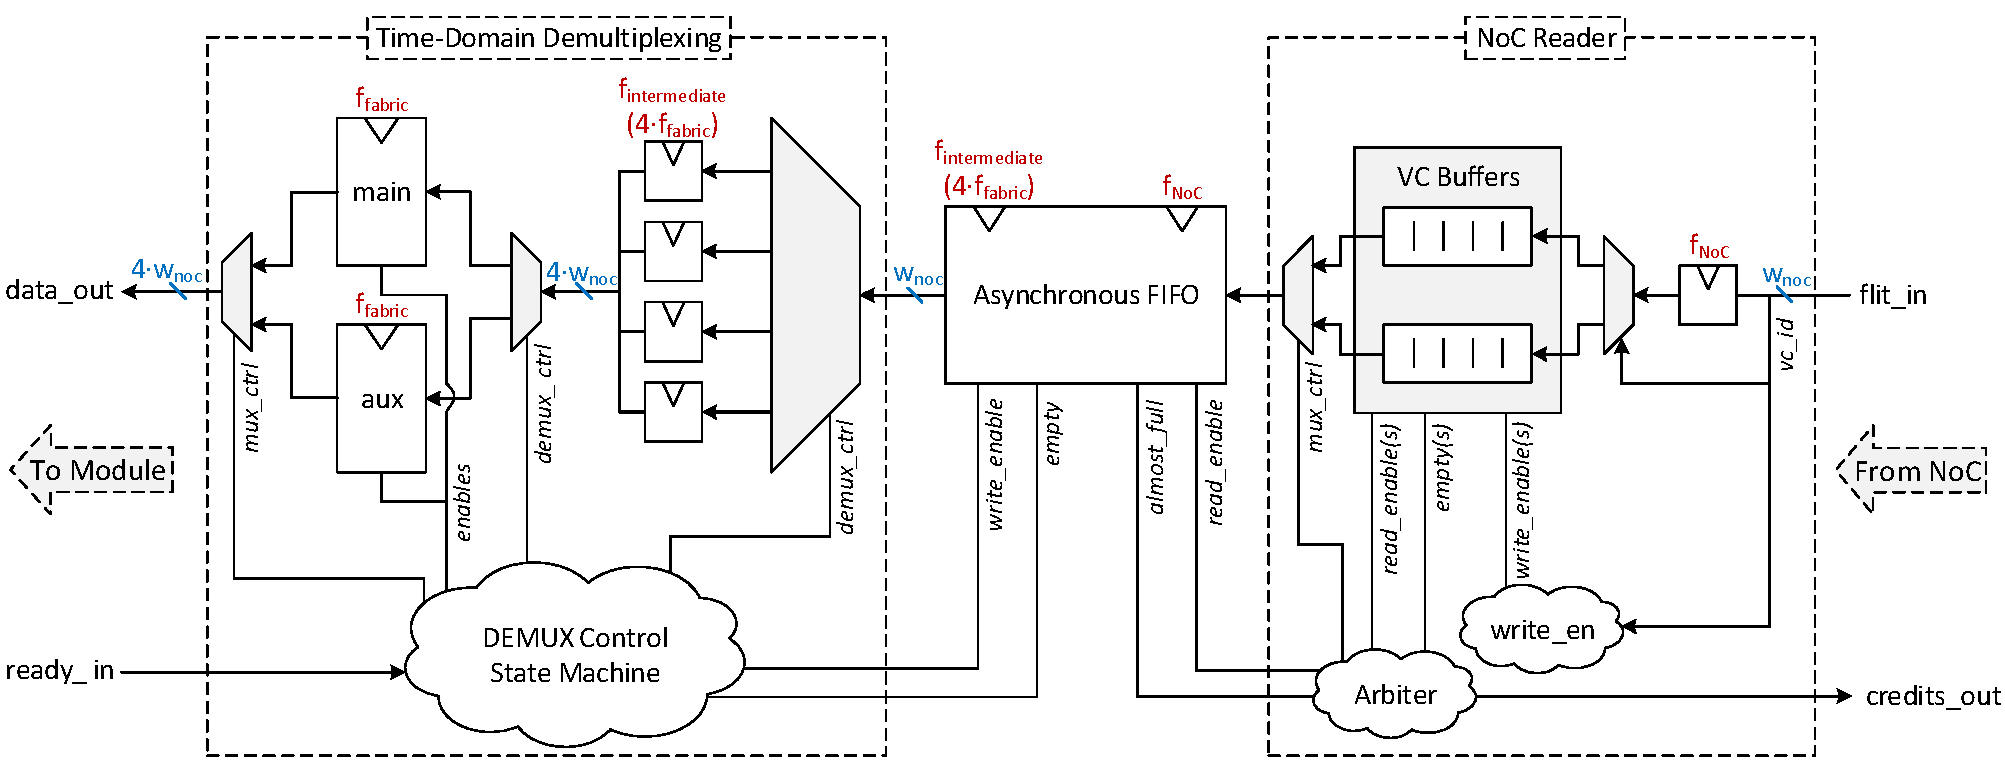
\includegraphics[width=2\columnwidth,keepaspectratio]{images/fpout_detail}
   \label{fpout}
 }
\caption{The FabricPort interfaces the FPGA fabric to an embedded NoC in a flexible way by bridging the different frequencies and widths as well as handling backpressure from both the FPGA fabric and the NoC.}
\label{fabric_port}
\end{figure*}

%----------------------------------------------------------------------------
\subsubsection{FabricPort Input: Fabric$\rightarrow$NoC}
%----------------------------------------------------------------------------

Fig.~\ref{fabric_port} shows a schematic of the FabricPort with important control signals annotated.
The FabricPort input (Fig.~\ref{fpin}) connects the output of a module in the FPGA fabric to an embedded NoC input.
Following the diagram from left to right: data is input to the time-domain multiplexing (TDM) circuitry on each fabric clock cycle and is buffered in the ``main" register.
The ``aux" register is added to provide elasticity. Whenever the output of the TDM must stall there is a clock cycle before the stall signal is processed by the fabric module. 
In that cycle, the incoming datum may still be valid, and is therefore buffered in the ``aux" registers.
To clarify this ready-valid behavior, example waveforms are illustrated in Fig.~\ref{stall_protocol}.
Importantly, this stall protocol ensures that every stall (ready = 0) cycle only stops the input for exactly one cycle ensuring that the FabricPort input does not reduce throughput.

The TDM unit takes four flits input on a slow fabric clock and outputs one flit at a time on a faster clock that is 4\xx as fast as the FPGA fabric -- we call this the intermediate clock.
This intermediate clock is only used in the FabricPort between the TDM unit and the asynchronous FIFO (aFIFO) buffer.
Because it is used only in this very localized region, this clock may be derived locally from the fabric clock by careful design of circuitry that multiplies the frequency of the clock by four.
This is better than generating 16 different clocks globally through phase-locked loops, then building a different clock tree for each router's intermediate clock (a viable but more costly alternative).

The output of the TDM unit is a new flit on each intermediate clock cycle.
Because each flit has a valid bit, only those flits that are valid will actually be written in the aFIFO thus ensuring that no invalid data propagates downstream, unnecessarily consuming power and bandwidth.
The aFIFO bridges the frequency between the intermediate clock and the NoC clock ensuring that the fabric clock can be completely independent from the NoC clock frequency and phase.

The final component in the FabricPort input is the ``NoC Writer".
This unit reads flits from the aFIFO and writes them to the downstream NoC router.
The NoC Writer keeps track of the number of credits in the downstream router to interface to the credit-based backpressure system in the embedded NoC, and only sends flits when there are available credits.
Note that credit-based flow control is by far the most-widely-used backpressure mechanism in NoCs because of its superior performance with limited buffering~\cite{dally_book}.
%Each sender keeps count of the number of credits; the sender has a credit for each available downstream buffer location.
%Therefore, a sender will only send data if it has available credits (telling it that there is buffer space downstream). 
%The downstream buffer sends a credit upstream only when it has freed one of its buffer locations by forwarding a flit.

%
%----------------------------------------------------------------------------
\subsubsection{FabricPort Output: NoC$\rightarrow$Fabric}
%----------------------------------------------------------------------------
%

Fig.~\ref{fpout} details a FabricPort output; the connection from an NoC output port to the input of a module on the FPGA fabric.
Following the diagram from right to left: the first component is the ``NoC Reader".
This unit is responsible for reading flits from an NoC router output port and writing to the aFIFO.
Note that separate FIFO queues must be kept for each VC; this is very important as it avoids scrambling data from two packets.
Fig.~\ref{demux} clarifies this point; the upstream router may interleave flits from different packets if they are on different VCs. 
By maintaining separate queues in the NoC reader, we can rearrange flits such that flits of the same packet are organized one after the other.

The NoC reader is then responsible for arbitrating between the FIFO queues and forwarding one (entire) packet -- one flit at a time -- from each VC.
We currently implement fair round-robin arbitration and make sure that there are no ``dead" arbitration cycles.
That means that as soon as the NoC reader sees a tail flit of one packet, it has already computed the VC from which it will read next.
The packet then enters the aFIFO where it crosses clock domains between the NoC clock and the intermediate clock.

The final step in the FabricPort output is the time-domain demultiplexing (DEMUX).
This unit reassembles packets (or packet fragments if a packet is longer than 4 flits) by combining 1-4 flits into the wide output port.
In doing so, the DEMUX does not combine flits of different packets and will instead insert invalid zero flits to pad the end of a packet that doesn't have a number of flits divisible by 4 (see Fig.~\ref{demux}).
%This is very much necessary to simplify the output of the NoC into something that is understandable by designers thereby creating an abstracted view of the NoC without complicating design.
This is very much necessary to present a simple interface for designers allowing them to connect design modules to the FabricPort with minimal soft logic.


%
\figvs{1}{demux}{}{``NoC Reader" sorts flits from each VC into a separate queue thereby ensuring that flits of each packet are contiguous. The DEMUX then packs up to four flits together and writes them to the wide output port but never mixes flits of two packets.}
%

%
%------------------------------------------------------------------------------------------------------------------------------
\subsection{FabricPort Discussion}
%------------------------------------------------------------------------------------------------------------------------------
%

%
%----------------------------------------------------------------------------
\subsubsection{Module Connectivity}
%----------------------------------------------------------------------------
%

The FabricPort converts 22.5~GB/s of NoC link data bandwidth (150~bits, 1.2~GHz) to 600~bits and any fabric frequency on the fabric side.
An FPGA designer can then use any fraction of that port width to send data across the NoC.
However, the smallest NoC unit is the flit; so we can either send 1, 2, 3 or 4 flits each cycle.
If the designer connects data that fits in one flit (150~bits or less), all the data transported by the NoC is useful data.
However, if the designer want to send data that fits in one-and-a-half flits (225~bits for example), then the FabricPort will send two flits, and half of the second flit is overhead that adds to power consumption and worsens NoC congestion unnecessarily.
Efficient ``translator" modules (see Fig.~\ref{fp_logical}) will therefore try to take the flit width into account when injecting data to the NoC.

\comment{
Note that the FabricPort's width is limited to 600 bits for our NoC and 20 bits of those will be used for control, leaving 580 bits for the designer to connect to their design modules.
Datapaths that are wider than 580 bits must be serialized through extra soft logic.


One clear limitation of the FabricPort is that the width is limited to 600 bits for our NoC and 20 bits of those will be used for control, leaving 580 bits for the designer to connect to their design modules.
Datapaths that are wider than 580 bits must be serialized through extra soft logic.
}


A limitation of the FabricPort output is observed when connecting two modules.
Even if each module only uses half the FabricPort's width (2 flits), only one module can receive data each cycle because the DEMUX only outputs one packet at a time by default as Fig.~\ref{demux} shows.
To overcome this limitation, we create a \textit{combine-data} mode as shown in Fig.~\ref{merge}.
For this combine-data mode, when there are two modules connected to one FabricPort, data for each module must arrive on a different VC.
The NoC Reader arbiter must strictly alternate between VCs, and then the DEMUX will be able to group two packets (one from each VC) before data output to the FPGA.
This allows merging two streams without incurring serialization latency in the FabricPort.
%
\begin{cond}
To combine packets at a FabricPort output, each packet must arrive on a different VC.
\end{cond}
%
Note that we are limited to the merging of two packets with 2 VCs but we can merge up to four 1-flit packets if we increase the number of VCs to four in the embedded NoC.
%Previous work has also identified the importance of merge functionality for FPGA applications and proposed creating NoCs out of split-merge primitives~\cite{Kapre2006}.

%
\figvs{1}{merge}{}{FabricPort output merging two packets from separate VCs in \textit{combine-data} mode, to be able to output data for two modules in the same clock cycle.}
%

%
%----------------------------------------------------------------------------
\subsubsection{Frequency and Latency}
%----------------------------------------------------------------------------
%


Fig.~\ref{zl_latency} plots the zero-load latency of the NoC (running at 1.2~GHz) for different fabric frequencies that are typical of FPGAs.
We measure latency by sending a single 4-flit packet through the FabricPort input$\rightarrow$NoC$\rightarrow$FabricPort output.
The NoC itself is running at a very fast speed, so even if each NoC hop incurs 4 cycles of NoC clocks, this translates to approximately 1 fabric clock cycle.
However, the FabricPort latency is a major portion of the total latency of data transfers on the NoC; it accounts for 40\%--85\% of latency in an unloaded embedded NoC.
The reason for this latency is the flexibility offered by the FabricPort -- we can connect a module of any operating frequency but that incurs TDM, DEMUX and clock-crossing latency.
Careful inspection of Fig.~\ref{zl_latency} reveals that the FabricPort input always has a fixed latency for a given frequency, while the latency of the FabricPort output varies by one cycle sometimes -- this is an artifact of having to wait for the \textit{next} fabric (slow) clock cycle on which we can output data in the DEMUX unit.
\comment{Additionally, the latency of the FabricPort is lowest at 300~MHz.
This is because 300~MHz is exactly one quarter of the NoC frequency, meaning that the intermediate clock is the same as the NoC clock and the aFIFO reads and writes flits at the same frequency, thus no additional clock-crossing latency is incurred.}


%
%
